\section{Atom in a damped cavity}

An application of the mathematical framework developed above is the study of the evolution of a single two-level atom initially prepared in the upper level $\ket{a}$ of the transition resonant with the cavity mode. In particular, it is seen that the spontaneous emission rate of the atom inside a resonant cavity is substantially enhanced over its free-space value (Purcell effect).

\begin{figure}[h!]
	\centering
	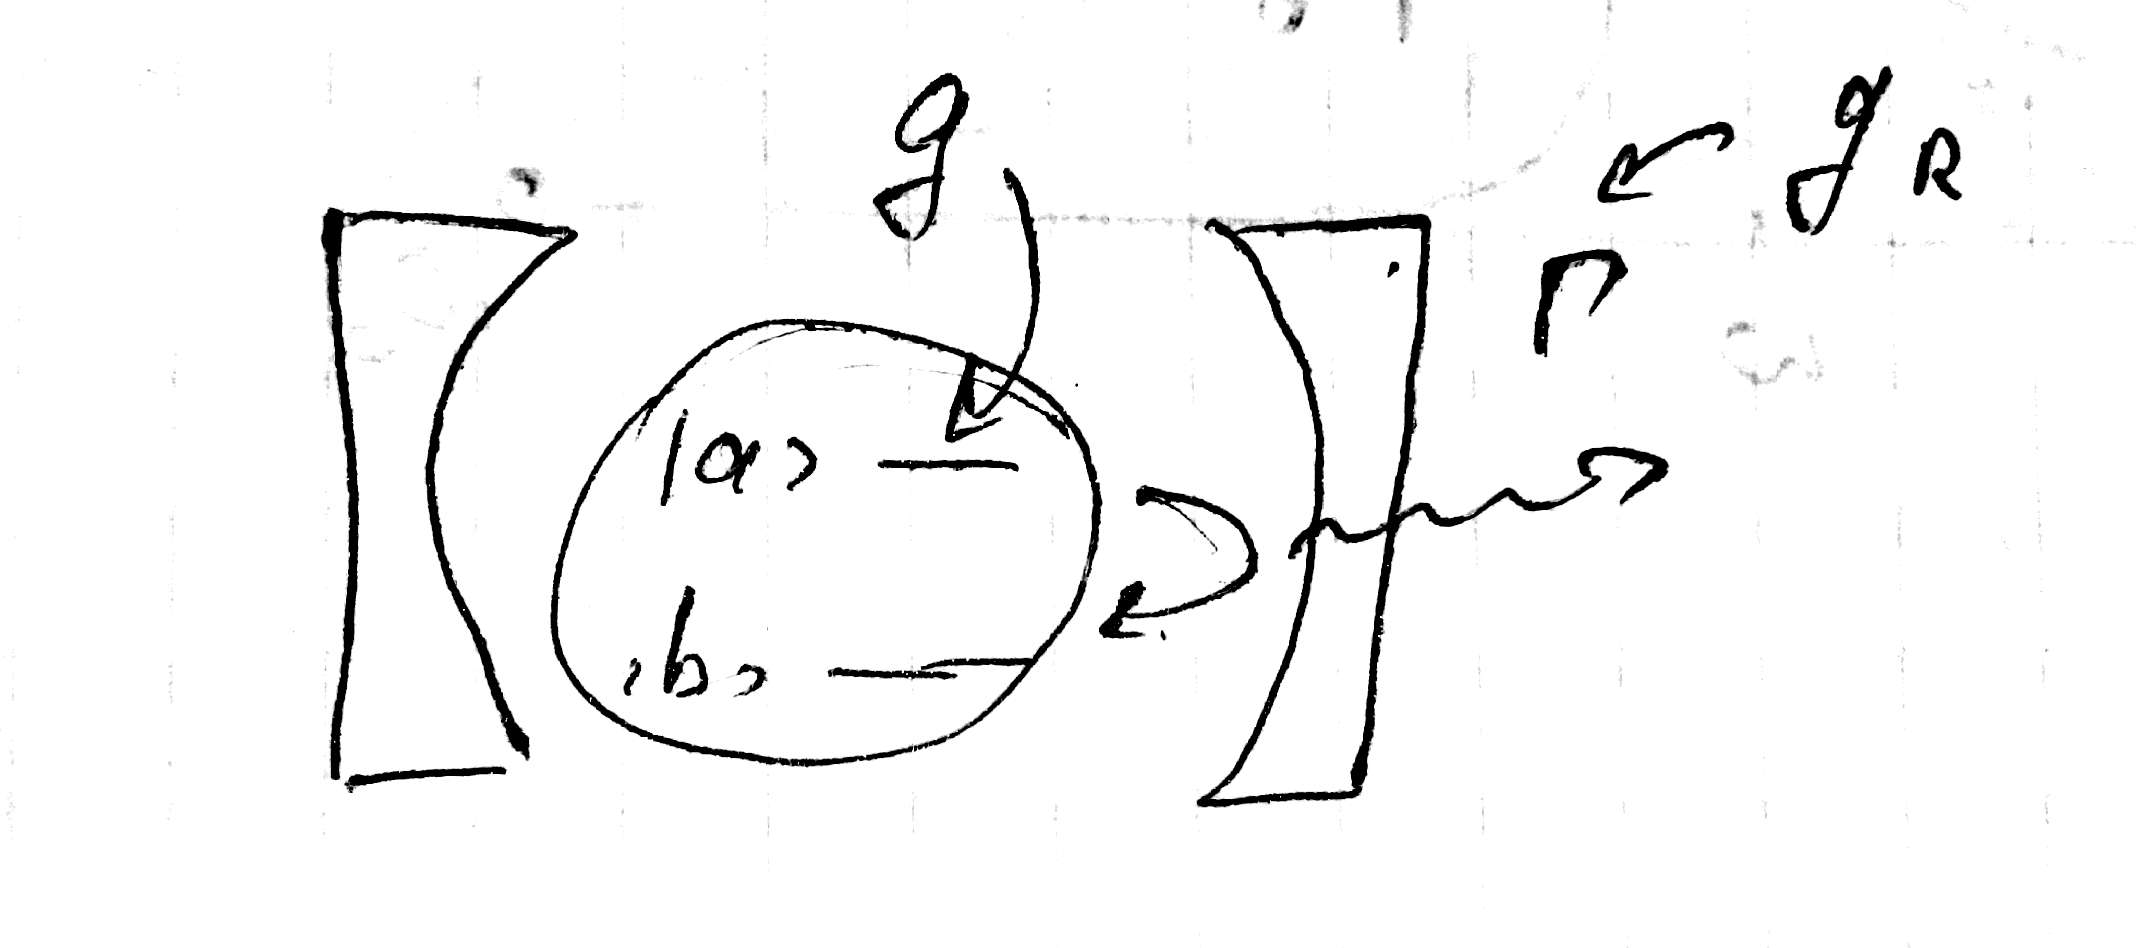
\includegraphics[width=0.4\linewidth]{fig/L10/atom_in_R}
	\caption{Atom in a cavity with losses. System has two coupling constants: $g$ --- atom and field coupling, $g_R$ --- cavity and reservoir coupling (transparency of a mirror)}
	\label{fig:atominr}
\end{figure}

\subsection{The Purcell factor for a closed cavity}

The decay rate $\gamma$ can be written as
\begin{equation}
	\gamma = 2 \pi \left| g(\omega) \right|^2 \frac{D(\omega)}{V},
	\label{eq:gamma}
\end{equation}
where $\rho = D/V$ is the density of state. In vacuum it is $D_0(\omega) = \frac{\omega^2}{\pi^2 c^3}$ but in a cavity it can be approximated by the Lorentzian (fig) with resonant frequency $\omega_0$
\begin{equation}
	D(\omega) = \frac{1}{\pi} \frac{\omega_{0}/2Q}{(\omega - \omega_{0})^2 + \left( \omega_{0}/2Q \right)^2}.
\end{equation}

\begin{figure}
	\centering
	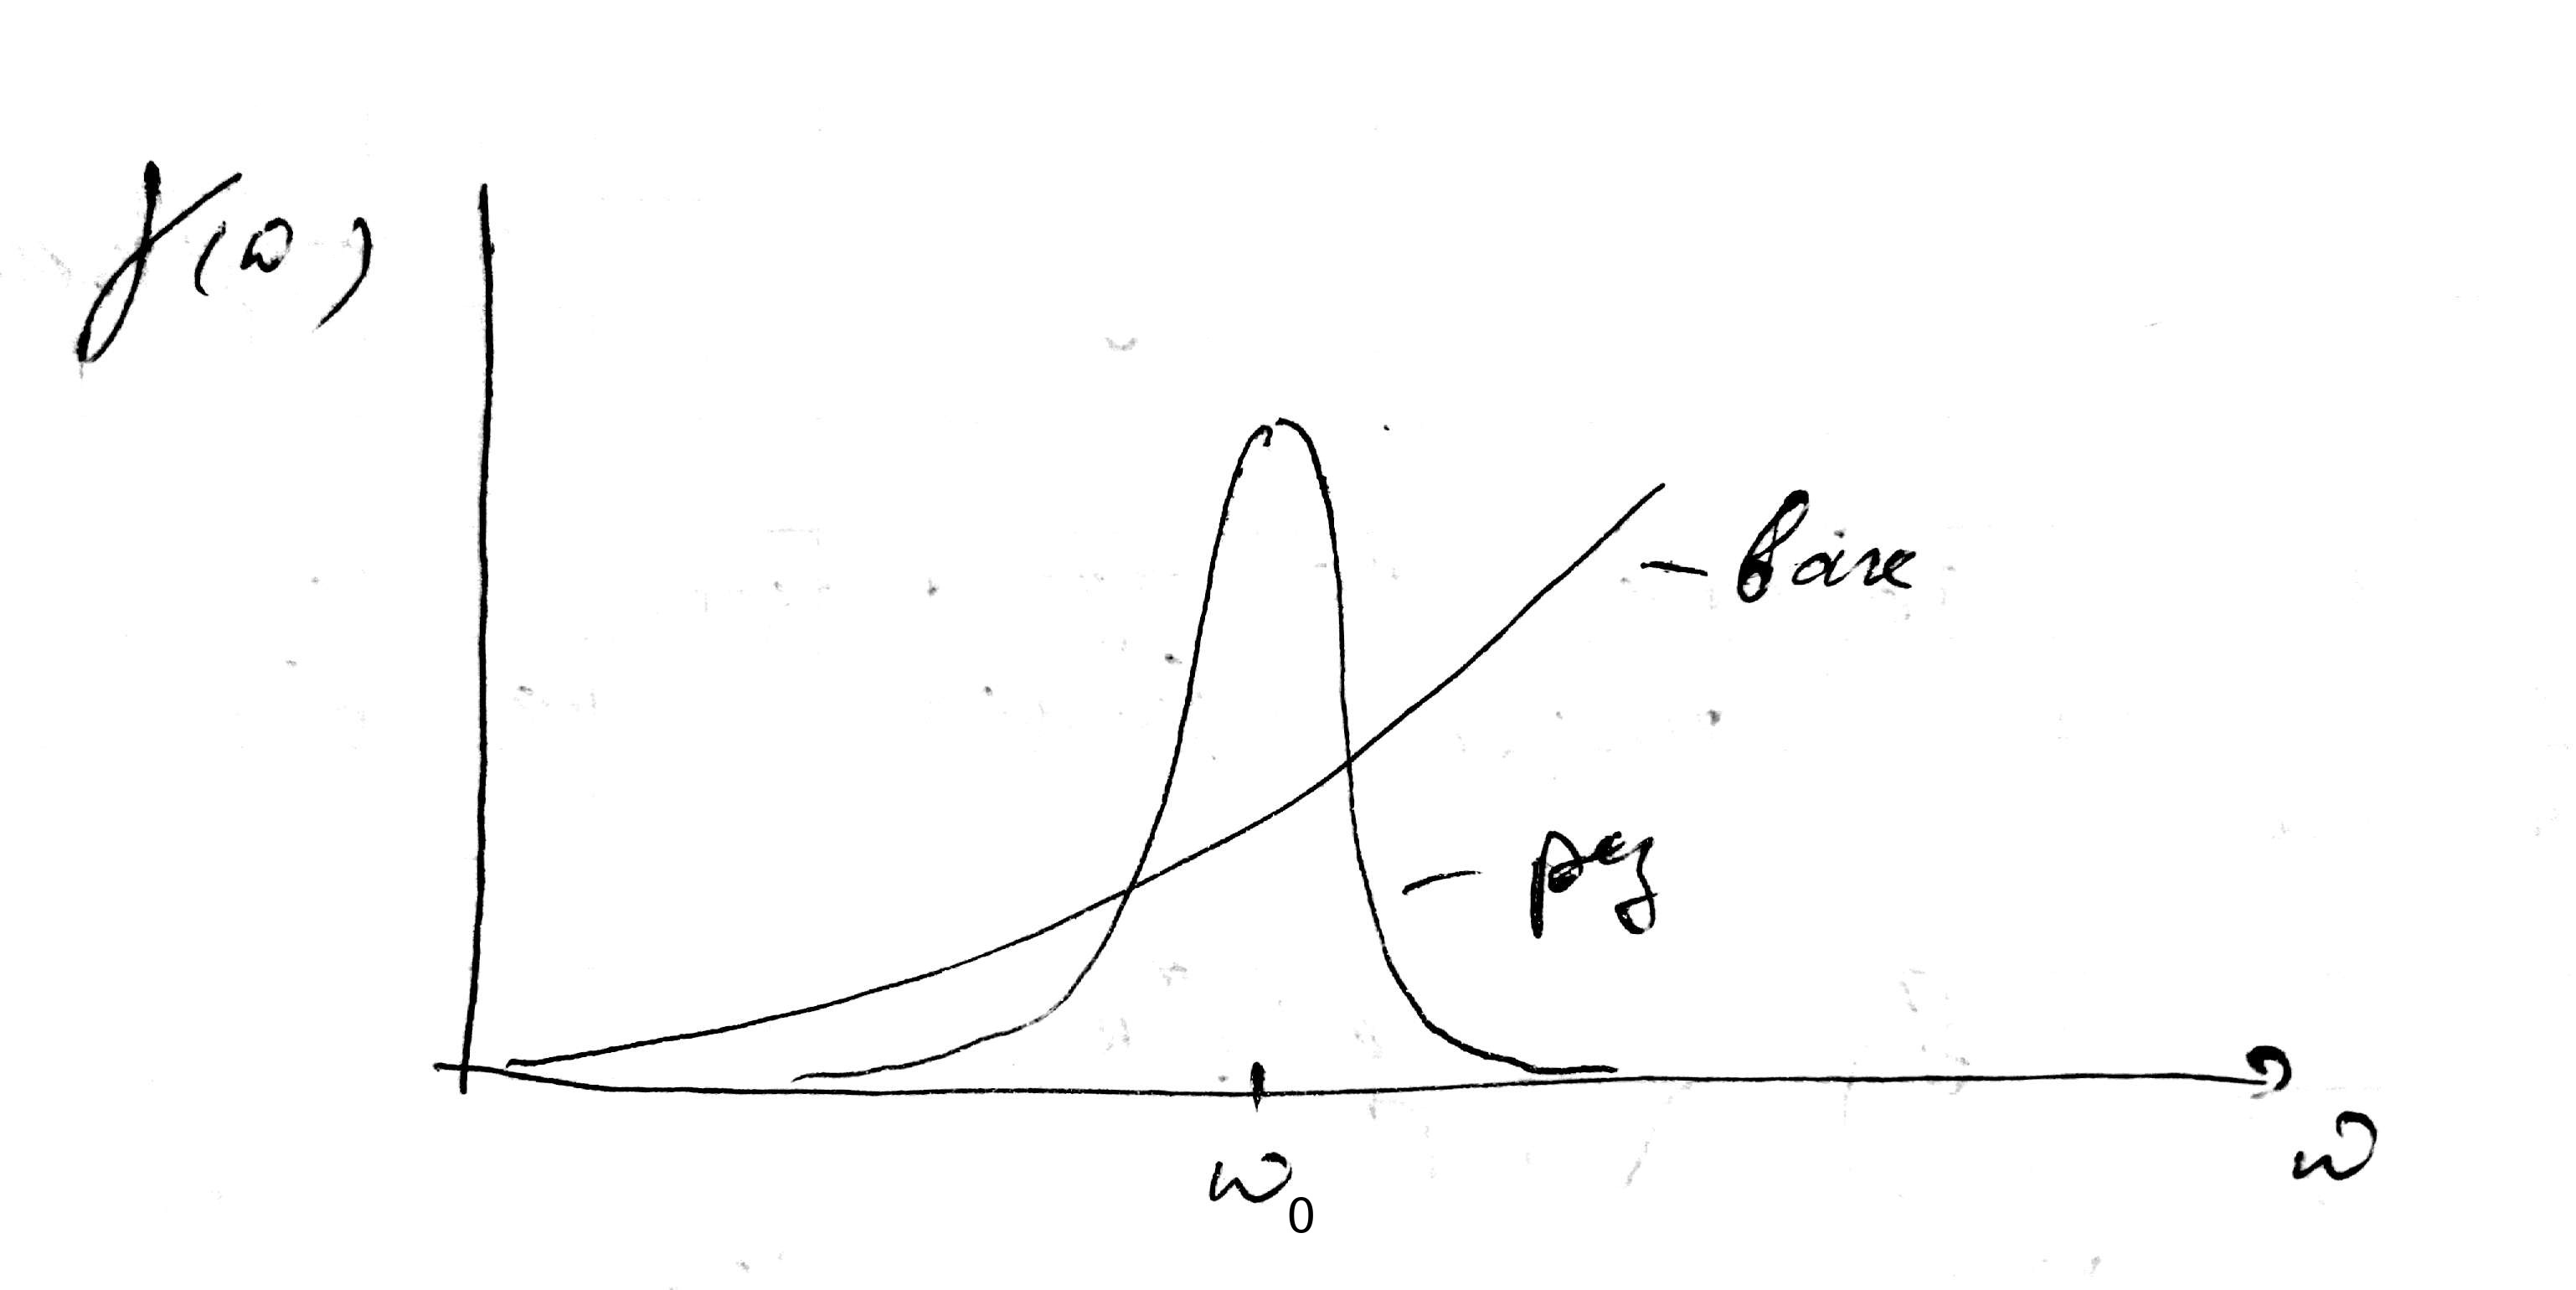
\includegraphics[width=0.5\linewidth]{fig/L10/gamma}
	\caption{The decay rate in vacuum and in a cavity}
	\label{fig:gamma}
\end{figure}

There two cases which is interesting to consider:
\begin{enumerate}
	\item[\textit{Case 1.}] $\omega \approx \omega_0$ --- transition and cavity frequencies are approximately equal. Then
	\begin{equation}
		D(\omega = \omega_0) \approx \frac{1}{\pi} \frac{2Q}{\omega_0}.
	\end{equation}
	Substitution to \eqref{eq:gamma} gives
	\begin{equation}
		\gamma = 2\pi \left| g(\omega) \right|^2 \frac{2Q}{\pi \omega} \frac{1}{V} = \underbrace{2\pi \left| g(\omega) \right|^2 \frac{\omega^2}{\pi^2 c^3}}_{\hookrightarrow=\gamma_0} \cdot \frac{1}{V} \frac{\pi^2 c^3}{\omega^2} \cdot \frac{2Q}{\pi \omega} = \gamma_0 \frac{1}{\left(2\pi\right)^2} \frac{\lambda^3}{V} Q,
	\end{equation}
	so the Purcell factor for a cavity is strongly depends on the $\lambda^3/V$ and the quality factor $Q$:
	\begin{equation}
		\boxed{F_{\text{P}} = \frac{\gamma}{\gamma_0} = \frac{1}{\left(2\pi\right)^2} \cdot \frac{\lambda^3}{V} Q.}
	\end{equation}
	
	\item[\textit{Case 2.}] $\left|\omega_0 - \omega\right| \gg \Gamma = \omega_0 / Q$. In this case we have
	\begin{equation}
		D(\omega) \approx \frac{1}{\pi} \frac{\Gamma}{2 \omega^2} = \frac{1}{2\pi} \frac{1}{Q \omega},
	\end{equation}
	then
	\begin{equation}
		F_{\text{P}} = \frac{\gamma}{\gamma_0} = \frac{1}{\left(2\pi\right)^2} \frac{\lambda^3}{V} \cdot \frac{1}{Q}.
	\end{equation}
	Usually $Q \gg 1$ and $\frac{\lambda^3}{V} \sim 1$, so far from the resonance $F_{\text{P}} \ll 1$.
\end{enumerate}

\subsection{Rigorous derivation of the atomic decay}